\acknowledgements{
\addtocontents{toc}{\vspace{1em}}  % Add a gap in the Contents, for aesthetics

\begin{figure}
    \centering
    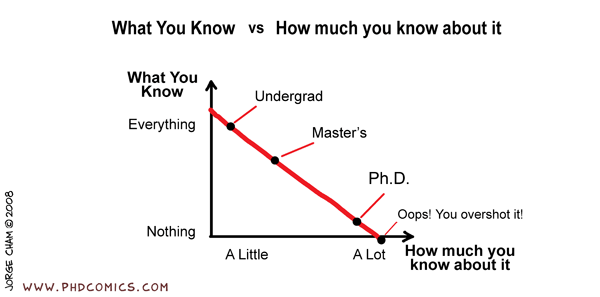
\includegraphics[width=0.7\linewidth]{Figures/comic.png}
\end{figure}

A common joke made about completing a PhD is that it teaches you a great deal about an insignificantly tiny slice of a field.
I would like to think I've come out a bit better than that (I know slightly less than a great deal about at least two tiny slices of chemistry), which I attribute almost entirely to my supervisor, Jonathan White.
I was lucky enough to stumble (literally, after a 21\textsuperscript{st} birthday the night before) into his group as a na\i{}ve Masters student, where I was immediately struck by the diversity of projects and people in the group.
From radiochemistry to photovoltaics, it seemed Jonathan could do anything.
I tried to imbibe as much of this attitude as I could during my Masters and PhD, sometimes ending up with a bit too much on my plate.
Nonetheless, thanks to Jonathan's wise counsel, I was able to tie almost all of the loose ends and disparate projects into this thesis.
I think this hunger for knowledge and eye for serendipity is one of the greatest gifts a supervisor could bestow on a PhD student, and for this I thank him profusely.

I also thank my PhD committee members, Brendan Abrahams and Uta Wille.
I genuinely looked forward to and enjoyed our annual progress meetings.
You both always provided such wonderful ideas and tangents for my projects, which I would never have otherwise thought of pursuing.
Along with Jonathan, you both helped to expose me to your respective areas of expertise, and I look forward to taking some of that knowledge with me to my first post-doc role.
Of course I shouldn't need to mention the incredible support and kindness you showed me.
I suppose I'm lucky I never had to, but I wouldn't have hesitated to come to either of your with any issues.
So thank you both, I couldn't have done it without you.

I owe a great deal to Colin Skene, for all the hands-on training throughout my Masters.
He also taught me the value of scientific rigour and detailed record-keeping, which I've tried to maintain as best as I can.

To all the members of the White group, past and present, thank you.
It's been an honour to work alongside such accomplished scientists, and your friendship is truly appreciated.
A special mention for the honorary White Walkers, Michael Ricca and Tze Cin Owyong, who have been a perpetual source of good times.
I will greatly miss our nights at Naughton's.

I thank all the wonderful friends I've made in the School of Chemistry.
Pre-COVID Friday Frothies were a monthly highlight, and the kick-ons to whichever watering hole happened to be open always reassured me that I had fallen into an excellent cohort.
On that note, I should also thank all the bar staff at Naughton's, The Clyde, Bobbie Peel's, and The Castle for so tactfully dealing with us rowdy chemists, and our heated late-night discussions over DFT functionals.

Thank you to my family, for 27 years of love and support, and for instilling in me the value of education.

Finally, I thank my loving partner, Alex Cummaudo.
You've taught me so much throughout our time together, not just about \LaTeX{}, but about persistence, compromise, and the value of family.
I'm so proud that I got to complete my PhD side by side with you, and I look forward to many more years with you and Pickles 
\includegraphics[width=1em]{Figures/pickles.png}.
}